\chapter{Discussion}

\phantomsection
\section*{Toxicity dataset}
\addcontentsline{toc}{section}{Toxicity dataset}

The dataset exhibited an imbalance towards the inactive compounds as shown in Figure \ref{fig:bars_endpoints}. This imbalance has significant implications for the clustering of active labels, as they are less prevalent. This observation is consistent with the occurrence of negative results in toxicity assays, where most of the tested compounds tend to be inactive. The endpoint with the highest ratio of active to inactive labels was SR.ARE (0.197), indicating a relatively higher response for this endpoint. Conversely, the lowest ratio was observed for NR.PPAR.gamma (0.032), suggesting a lower response to the test. Nevertheless, SR.ARE is also one of the endpoints having the highest missing values ratio. The scarcity of active chemicals and missing values can impact the overall performance of the subsequent analysis and should be considered while interpreting the results.

High correlation was found for some endpoints. The phi coefficient is a measure of association between two binary variables, indicating the strength and direction of the relationship. In Figure \ref{fig:phi_coefficient}, the phi coefficients reveal the extent of similarity between various pairs of endpoints. The high phi coefficients for NR.AR - NR.AR.LBD (0.76) and NR.ER - NR.ER.LBD (0.74) indicate a strong positive association between these pairs, suggesting a close relationship and similarity in their binary classifications and it could explain their similar predictions. These two pairs of assays are usually correlated because of their similar objectives, the first pair are related to the androgen receptor and the second one to the estrogen receptor. For example, if a chemical can bind to the ligand binding domain (LBD) of the androgen receptor (AR) (labelled as active for the NR.AR.LBD endpoint), then is very likely that the binding can affect the conformation and activity of the androgen receptor, which lead to a positive result for the NR.AR endpoint.


\phantomsection
\section*{Spectra in MassBank library}
\addcontentsline{toc}{section}{Spectra in MassBank library}

In the dataset, small molecules are predominant as shown in Figure \ref{fig:library} (a). This observation aligns with the general understanding that smaller molecules have a higher potential to penetrate biological barriers and interact with cellular processes, which can impact their bioactivity and toxicity. Small molecules are also predominant in toxicity datasets, e.g., drugs and pesticides. However, it is worth noting that the relationship between molecular mass and toxicity is much more complex involving various mechanisms. For instance, the big carbohydrate-binding protein ricin (64-65 kDa) can also penetrate biological barriers and disrupt protein synthesis within cells leading to toxicity \cite{SANDVIG2000415}. 

This collection of spectra constitues the chemical space that is explored in the scope of this study. The understanding of these boundaries is important to interpret the prediction capabilities of this approach.


\phantomsection
\section*{Spectra similarity}
\addcontentsline{toc}{section}{Spectra similarity}


\phantomsection
\subsection*{Mapping cosine}
\addcontentsline{toc}{subsection}{Mapping cosine}
From all pairwise comparisons, 1185 (0.13\%) pairs exhibited a cosine similarity greater than 0.5, while only 139 pairs had a cosine greater than 0.7, as detailed in Table \ref{table:frequency_cosine}. Some possible factors leading to a small number of highly similar pairs could be the intrinsic structural similarity of the dataset and the similarity metric for the combined spectra .  

The similarity across the dataset shows certain characteristics highlighted in Figure \ref{fig:cosine}. Some spectra exhibited broad similarities with the rest of the dataset, as can be seen by the transversal marks at the bottom and right  parts. This could be in part due to the greater amount of analytical information. As multiple collision energies are available in the library, the number of total peaks and matched peaks increases. For example, cortisol has the highest mean similarity with all the compounds (0.127, the global mean is 0.0428) and has 26 different mass spectra (the average is 11.7 spectra per compound). Certain molecules were more similar within specific groups, forming clusters, as seen in the lower right corner of Figure \ref{fig:cosine}. The upper part of the diagonal indicates the presence of multiple smaller groups. In contrast, the dark cross region, originating from the center of the axis, indicates subsets with low similarity. In general, the heatmap shows groups of spectra with shared similarity where the network can be built, as it be will further explored later.

The cosine similarity is a widely utilized metric for assessing the similarity between spectra. In principle, having a greater amount of empirical information can be beneficial for associating structures and predicting bioactivity, such as shared toxophores between compounds. Having more peaks, obtained from different ionization energies, can assist in identifying coincidental fragments. However, the cosine similarity can be susceptible to the influence of isotopic peaks, noise, or background interference. When confronted with a large number of peaks, including noise or isotopic peaks, the cosine score may decrease as the vector lengths increase. In such cases, the cosine similarity may yield low scores, potentially leading to erroneous assessments of structural similarity.

Some alternatives for calculating similarity between spectra with high density of peaks would be computing a consensus spectra per InChIKey and machine learning-based scores. A consensus spectra would cluster the peaks across \textit{m/z} and assign an intensity based on their frequency on the library. This approach would significantly reduce the number of peaks per spectra and have the potential of improving the performance of cosine similarity. Additionally, a machine learning-based score can select the fragments that contain certain structural information by recognizing patterns across the spectra dataset. These two alternatives are further discussed later in the networking section. 

In general, the cosine scores alone for the combined spectra provided a satisfactory number of pairs for networking and demonstrated sufficient structural similarity upon examination of the pairs. This study specifically focused on the application of cosine similarity, which will be discussed in more detail in the following sections.

\phantomsection
\subsection*{Pairwise comparison}
\addcontentsline{toc}{subsection}{Pairwise comparison}

After analyzing the cosine map, the pairwise comparison were explored in more detail. For this, the number of matched peaks was examined for its relationship with the cosine score in Figure \ref{fig:cosine_ij}. From this graph, it can be seen the density of pairs sharing certain levels of similarity, this would be helpful later to interpret the networks.

The scores are concentrated on the lower left part of Figure \ref{fig:cosine_ij}. Conversely, the upper part of the graph exhibits a low-density area containing pairs with sufficient similarity to establish nodes in the spectral networks. On the left side of the graph, low number of matched peaks can exhibit also high similarities; while on the right side of the graph, large number of matched peaks (and consequently total peaks) are less likely to have very low cosine scores. 

The right upper region, sparsely populated, represents a highly similar mass spectra where the number of matched peaks is close to the total number of peaks. For instance, the right farthest pair has a cosine value of 0.54 and 1062 matched peaks. This pair consists of colchicine and prednisone, both medications. These substances are well-documented in the MassBank library, with 39 and 40 spectra, respectively. Moreover, their complex fragmentation patterns are evident from the number of peaks per spectrum, surpassing 100 peaks in some cases. The presence of several fused rings and functional groups in both molecules results in multiple fragmentation pathways, contributing to the high number of matched peaks. However, their cosine similarity is relatively low partly because of the increase in the lenght of the vectors. This is an example that even at high number of matched peaks, the abundance of peaks can be detrimental for the cosine score. Most of the high cosine values are, in fact, found at a low number of matched peaks.


%%%%%%%

\phantomsection
\subsection*{Cosine budget}
\addcontentsline{toc}{subsection}{Cosine budget}

Some spectra share similarities across the dataset more than others. The cosine budget is here presented as the sum of all the cosine values of a spectra. A high cosine budget indicates that similarities are shared over a wide range of spectra, while a low cosine budget represents narrowed similarity and specificity. Some factors that are related to the cosine budget are number of available spectra, total peaks per spectra and total matched peaks, which are described below.

\subsubsection*{\textit{Number of spectra}}

The increase of the number of spectra in the library is more likely to yield high cosine budgets until a certain point, as shown in Figure \ref{fig:sum_cosine_vs_spectra}. This could be explained by the increase in empirical analytical information (e.g., more fragments as result of more collision energies in the library) that results in the identification of additional common peaks. However, the graph also shows a negative effect at high number of available spectra. High abundance of multiple mass spectra for a compound shows less frequency of high cosine budgets. This could be explained by the negative effect of noise features in the cosine similarity measure. Moreover, it could correspond to a cosine budget threshold, for which the increment of spectra do not provide additional fragment information that can be shared within the dataset. 

\subsubsection*{\textit{Total number of peaks}}

Some mass spectra can have a high number of peaks, in some cases more than a hundred. Therefore, the total number of peaks per InChIKey across the dataset and its relationship with cosine was investigated. The combined spectra contain all the peaks associated with an InChIKey. A greater amount of peak information tends to have a greater cosine budget as it is shown in Figure \ref{fig:cross_cosine}. The graph shows high density of compounds in the lower matched peaks and cosine budget suggesting low similarities within the dataset and therefore low clustering tendencies for those chemicals. On the upper right part, there are fewer and dispersed compounds with high similarity across the dataset more likely to be in clusters.

The dispersion of cosine budget is higher as the number of peaks increases. High cosine similarity budget could reflect structural features that are common in the chemical space of the dataset. A high number of peaks can be due to complex fragmentation patterns and a greater availability of mass spectra in the library. The ten highest cosine budgets are for the chemicals described in Table \ref{table:cross_cosine}. Steroids and other cyclic compounds are predominant chemical structures. Steroids are structural complex and have multiple rings and functional groups. Hydroxyl (-OH), carbonyl (C=O) groups, and double bonds provide different sites for bond cleavage, leading to diverse fragmentation pathways and resulting in multiple peaks. Additionally, the fused ring system can be fragmented in one or more rings and produce different fragment ions. Other factor is that the isomeric structures (e.g., positional and stereoisomers) can contribute to the generation of multiple peaks. The complex complex nature of steroids could also explain their high cosine budgets and their location in the spectral network. The dispersion of cosine budget is higher as the number of peaks increases. High cosine similarity budget could reflect structural features that are common in the chemical space of the dataset. A high number of peaks can be due to complex fragmentation patterns and a greater availability of mass spectra in the library. The ten highest cosine budgets are for the chemicals described in Table \ref{table:cross_cosine}. Steroids and other cyclic compounds are predominant chemical structures. Steroids are structural complex and have multiple rings and functional groups. Hydroxyl (-OH), carbonyl (C=O) groups, and double bonds provide different sites for bond cleavage, leading to diverse fragmentation pathways and resulting in multiple peaks. Additionally, the fused ring system can be fragmented in one or more rings and produce different fragment ions. Other factor is that the isomeric structures (e.g., positional and stereoisomers) can contribute to the generation of multiple peaks. The complex complex nature of steroids could also explain their high cosine budgets and their location in the spectral network. 

% cross_cosine.csv < .odt
\begin{sidewaystable}[p]
 \centering
\footnotesize
\caption{Compounds with the highest cosine budgets}
\label{table:cross_cosine}
%\begin{tabular}{||l l l l l l l l||}
\begin{tabular}{||c c c c c c c c||}
\hline
Compound & Structure & Formula & Exact mass (Da) & No. of spectra & No. total of peaks & Cosine budget & Normalized cosine budget\\ [0.5ex]
\hline
\hline
Danazol&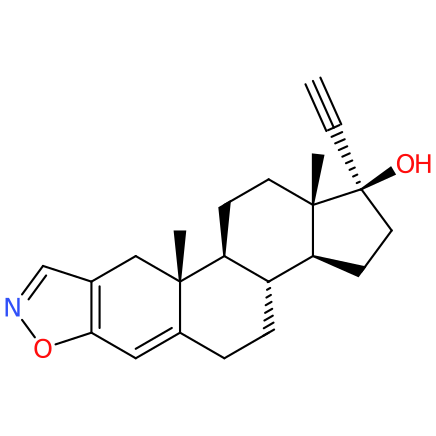
\includegraphics[width=1cm]{include/img/results/topcosine/Danazol.pdf}&\ce{C22H27NO2}&337.2042&6&302&200.9&1.00\\
Resibufogenin&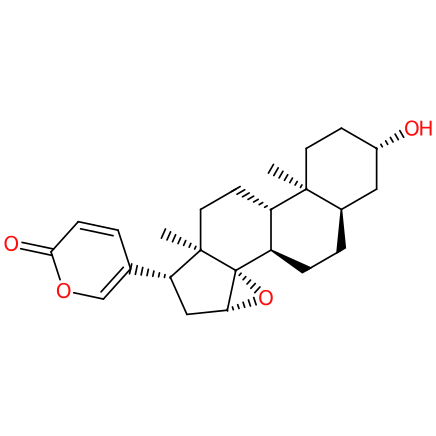
\includegraphics[width=1cm]{include/img/results/topcosine/Resibufogenin.pdf}&\ce{C24H32O4}&384.5160&10&439&188.18&0.94\\
Betamethasone valerate&\includegraphics[width=1cm]{include/img/results/topcosine/Betamethasone_valerate.pdf}&\ce{C27H37FO6} &476.2574 &6&354&186.8&0.93\\
Corticosterone&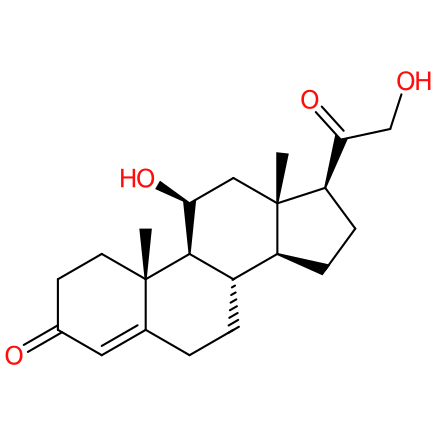
\includegraphics[width=1cm]{include/img/results/topcosine/Corticosterone.pdf}&\ce{C21H30O4}&346.2144&19&881&178.2&0.89\\
Etofenprox&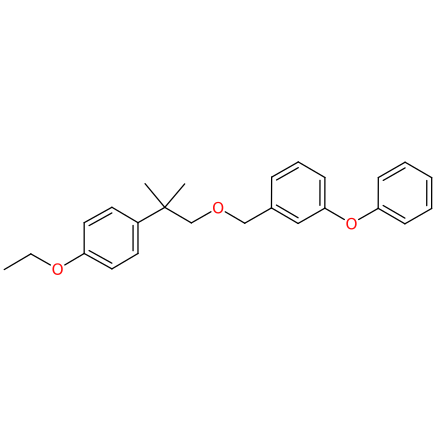
\includegraphics[width=1cm]{include/img/results/topcosine/Etofenprox.pdf}&\ce{C25H28O3}&376.2038 &6&309&177.6&0.89\\
Norethindrone&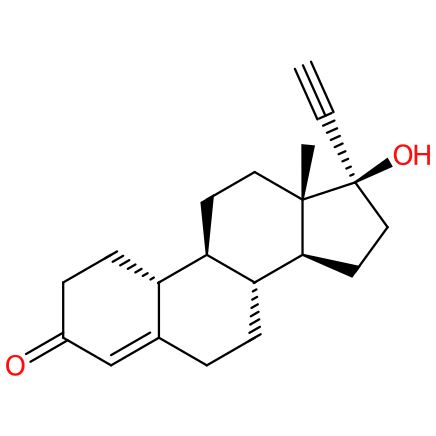
\includegraphics[width=1cm]{include/img/results/topcosine/Norethindrone.pdf}&\ce{C20H26O2} &298.1933&21&608&175.5&0.88\\
Gestoden&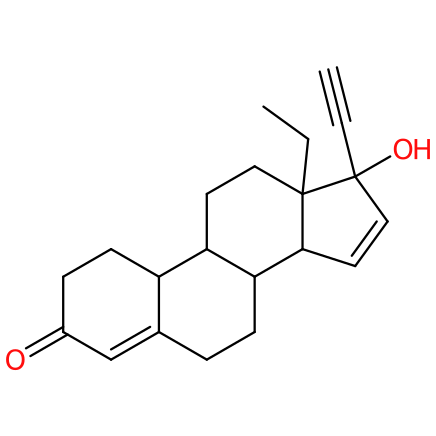
\includegraphics[width=1cm]{include/img/results/topcosine/Gestoden.pdf}&\ce{C21H26O2}&310.1933 &6 &421&175.3&0.88\\
Glycyrrhetinic Acid&\includegraphics[width=1cm]{include/img/results/topcosine/Glycyrrhetinic_Acid.pdf}&\ce{C30H46O4}&470.3396&34&379&175.2&0.88\\
Cyproterone acetate&\includegraphics[width=1cm]{include/img/results/topcosine/Cyproterone_acetate.pdf}&\ce{C24H29ClO4}&416.1754 &6&463&174.6&0.88\\
Betamethasone&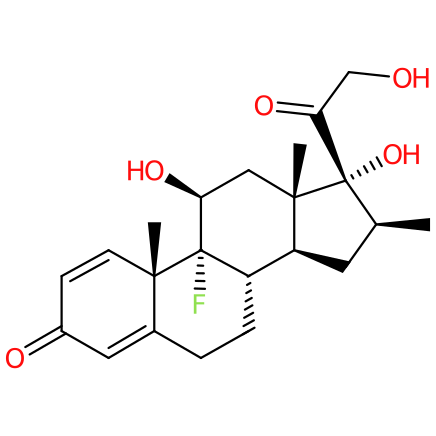
\includegraphics[width=1cm]{include/img/results/topcosine/Betamethasone.pdf}&\ce{C22H29FO5}&392.1999 &8&319&173. 5&0.86\\
[1ex]

 \hline
\end{tabular}
\end{sidewaystable}






\subsubsection*{\textit{Total number of matched peaks}}

The number of total matched peaks across the dataset is also an indication of clustering tendency. Figure \ref{fig:sum_cosine_vs_matched_peaks} illustrates the relation of matched peaks with tolerance 0.1 \textit{m/z} and the cosine budget. The x-axis shows the total number of peaks from all spectrums per unique InChIKey in mass spectra dataset after filtering. The y-axis represents the sum of all the cosine similarity of a chemical against the others in the dataset. The number of peaks represents the amount of analytical information available for a chemical. A higher dispersion of the cosine budget can be noticed at higher number of peaks. The cosine budget indicates the total similarity of a chemical with the dataset. Most of the spectra are concentrated in the lower left part of the scatter plot. This region constitutes the set of compounds that have low similarity with the chemical space, therefore will not be forming clusters in spectral networks. On the other side, the upper right corner of the graph captures the compounds that are more likely to form clusters as they have high cosine budget and high number of matched peaks across the dataset. However, the density in this region is low and this will be observed in the networks where only a small fraction of the dataset will establish clusters.


The combined effect of the total number of peaks and matched peaks is illustrated in Figure \ref{fig:circles_cosine}. The graph shows a random sample of 10 \% for better visibility. The x axis shows the total number of peaks that are available in the MassBank.eu for each InChIKey. The number of peaks can be read as an indication of the available peak information for a chemical. The y axis shows the total number of matched peaks of the chemical across all the dataset. The latter is an indication of shared features. Additionally, the circle size illustrates the cosine budget as the sum of all the cosine similarities of a chemical across the dataset. The trend in Figure \ref{fig:circles_cosine} shows that those chemicals that have a greater number of peaks in the library result in a greater cosine budget, which could be due to small cosine score and fragments shared across the dataset. 



\begin{figure}[htbp]
    \centering
    \begin{subfigure}[b]{0.49\textwidth}
        \centering
        \includegraphics[width=\textwidth]{include/img/results/sum_cosine_vs_spectra.pdf}
        \caption{}
        \label{fig:sum_cosine_vs_spectra}
        \vspace{0.1cm}
        \begin{minipage}[t]{\textwidth}
        \end{minipage}
    \end{subfigure}
    \hfill
    \begin{subfigure}[b]{0.49\textwidth}
        \centering
        \includegraphics[width=\textwidth]{include/img/results/sum_cosine.pdf}
        \caption{}
        \label{fig:sum_cosine_vs_matched_peaks}
        \vspace{0.1cm}
        \begin{minipage}[t]{\textwidth}
        \end{minipage}
    \end{subfigure}

%    \vspace{0.5cm} 

    \begin{subfigure}[b]{0.49\textwidth}
        \centering
        \includegraphics[width=\textwidth]{include/img/results/sum_cosine_vs_matched_peaks.pdf}
        \caption{}
        \label{fig:cross_cosine}
        \vspace{0.1cm}
        \begin{minipage}[t]{\textwidth}
        \end{minipage}
    \end{subfigure}
    \hfill
    \begin{subfigure}[b]{0.49\textwidth}
        \centering
        \includegraphics[width=\textwidth]{include/img/results/matched_peaks.pdf}
        \caption{}
        \label{fig:circles_cosine}
        \vspace{0.1cm}
        \begin{minipage}[t]{\textwidth}
        \end{minipage}
    \end{subfigure}
    \caption{(a) Relationship between the cosine budget and the number of spectra per InChIKey; (b) number of peaks and the cosine budget; (c) cosine budget and the sum of total matched peaks within a tolerance of 0.1 \textit{m/z};  (d) matched peaks, total number peaks, and the cosine budget.}
    \label{fig:22subfigures}
\end{figure}


\begin{figure}
    \centering
  \begin{minipage}[b]{0.9\textwidth}
    \centering
    \includegraphics[width=\textwidth]{include/img/appendix/net_structures/steroids.png}
    \subcaption{Steroids}
  \end{minipage}
  \hfill
  \begin{minipage}[b]{0.8\textwidth}
    \centering
    \includegraphics[width=\textwidth]{include/img/appendix/net_structures/phthalates.png}
    \subcaption{Phthalates}
  \end{minipage}
  \caption{Molecular structures of a subset of pairs with cosine similarity greater than 0.6. A wider edge represents a higher cosine score. The figure shows that the connected nodes have similar molecular structures. In the case of (a) steroids, the majority of the group shows activity, whereas (b) phthalates mostly are inactive for the NR.AR endpoint.}
  \label{fig:net_structures}
\end{figure}


\subsubsection*{\textit{Chemical class}}

Another aspect that could be responsible for the high cosine budget is the presence of chemical classes. Some predominant classes could explain the broad similarities that some chemicals share across the dataset. One indication of predominant classes is the clustering of steroids as shown Figure \ref{fig:NR.AR_class} and Figure \ref{fig:net_structures}. This aspect is discussed in the section of spectral networking. Steroids have a greater number of fragments compared to other chemical classes. The abundance of peaks increases the number of total matched peaks and cosine budget. Additionally, some compounds, e.g., as carboxylic acids and indoles, might receive lower scores using cosine similarity \cite{bittremieux_comparison_2022}. 




%#################
\subsubsection*{\textit{Combination of several spectra}}

The combination of several mass spectra can influence the cosine similarity. In this case, all the peaks from different mass spectra were combined. Then, the cosine function paired the matched peaks within a tolerance of 0.1 \textit{m/z}. Each peak can be paired only once. The effect of the matching tolerance was also explored and it is described in Table \ref{table:nets_opt}. A tolerance of  0.001 \textit{m/z} reduced the number of nodes to 235 and edges to 193, the resulting network is illustrated in Figure \ref{fig:net_0001}. 



%#################
\subsubsection*{\textit{Neutral losses}}
The occurrence of neutral losses can influence the cosine similarity by modifying the intensity and abundance of peaks. The measurement conditions, sample preparation, and the nature of the compound make it difficult to correctly identify all losses during fragmentation. The abundance of peaks is particularly increased in large molecules with several functional groups. For instance, steroids can exhibit neutral losses due to the hydroxyl attached to their fused rings. These losses lead to an increase in the number of peaks and it can result in lower cosine scores. Further investigation on accounting for neutral losses could have a positive effect on the accuracy of the similarity metrics.


%#################

\phantomsection
\subsection*{Deep learning-based similarity metric}
\addcontentsline{toc}{subsection}{Deep learning-based similarity metric}

Additionally, to the cosine similarity, a deep learning-based metric was examined for its ability to cluster similar molecules within a network. MS2DeepScore \cite{huber_MS2deepscore_2021} is a deep learning-based similarity score that uses convolutional neural networks to predict structural similarity scores. This score exhibited a more balanced distribution in comparison to the cosine similarity, as depicted in Figure \ref{fig:comparison_cosine_ms2ds}. This can be attributed to MS2DeepScore's ability to capture the complex relationships between mass spectra peaks.

\begin{figure}[h]
    \centering
	 \begin{subfigure}[b]{0.495\textwidth}
 		 \hspace{3cm}
 		 \centering
 		 \includegraphics[width=1\textwidth]{include/img/results/frequency_ms2ds_cosine.pdf}
 		 \caption{}
 	\end{subfigure}
 	\hfill
 		 \begin{subfigure}[b]{0.465\textwidth}
 		 \hspace{3cm}
 		 \centering
  		\includegraphics[width=1\textwidth]{include/img/results/frequency_ms2ds_cosine_05.pdf}
 		 \caption{}
 	\end{subfigure}
  \caption{Comparison of pairwise scores between cosine and MS2DeepScore for the whole range (a) and higher half (b).}
  \label{fig:comparison_cosine_ms2ds}
\end{figure}


In the higher range of the similarity scale (0.5 to 1), MS2DeepScore exhibited approximately 10 times more pairs compared to the cosine score as shown in Figure \ref{fig:comparison_cosine_ms2ds}. However, it is important to note that this disparity in pair counts does not directly imply a greater number of structurally similar pairs being identified. The calculation and interpretation of these two metrics are distinct. While MS2DeepScore may generate more pairs in this range, the interpretation and significance of those pairs may differ from those obtained using the cosine similarity.

Given the better explainability and interpretability of the cosine similarity, this study primarily focused on its exploration and analysis in the subsequent sections. The use of cosine similarity allows for a clearer understanding of the structural similarities between mass spectra, facilitating the interpretation of the results.

\phantomsection
\section*{Spectral similarity networks}
\addcontentsline{toc}{section}{Spectral similarity networks}
\label{sec:networks}
The cosine similarity, calculated in the previous section, was used to construct networks in the form of a graph. On the network, the nodes represent the combined spectra, each representing a unique compound identified by its InChIKey, and the edges represent the cosine similarity between the spectra. The topology of the spectral network is influenced by various factors, such as the minimum similarity required to form an edge between two nodes and the maximum number of connections a node can establish with other nodes.

The selection of the optimal network was based on a combination of statistical summaries and visual inspection. Key factors considered included the total number of nodes and edges, the average number of neighbors, characteristic path length, and clustering coefficient. These measures provide insights into the local connectivity patterns among mass spectra that are structurally or functionally similar. By examining the network statistics, it is possible gain a more objective description of the relationships in the spectra dataset.

For a detailed overview of the graph statistics under different conditions, please refer to Table \ref{table:nets_opt}. The table provides a summary of the network properties for various sets of conditions, allowing for a comparative analysis of the different network configurations. The effect of some of those conditions are further described below.

\subsubsection*{\textit{Effect of tolerance, minimum similarity and maximum edges}}

When applying a matching tolerance of 0.1 \textit{m/z}, the change from minimum cosine from 0.5 to 0.6 led to a change in the characteristic path length from 7.44 to 2.97 (-60\%). The improvement in the characteristic path length is relevant and denotes a more similar mass spectra in the network and interconnected structure with nodes closer to each other. This is slightly enhanced for cosine 0.7, giving a characteristic path length of 2.68 (-10\%). However, the number of nodes and edges are reduced by 50\% and  60\%, respectively. In similar way, the average number of neighbors went down from 6 to 3. The clustering coefficient slightly increased and suggested neighboring nodes densely interconnected in local clusters. 

For matching peaks with a tolerance of 0.001 \textit{m/z}, there were fewer nodes and edges compared to the 0.1 \textit{m/z} tolerance at the respective cosine, cut-offs as shown in Table \ref{table:nets_opt} and in Figure \ref{fig:net_0001}. This reduction of nodes could be benefitial as it increased the clustering coefficient and peak matching pairing accuracy; however, the chemical space is also reduced which could be detrimental for connecting unseen spectra with the network. The characteristic path length was slightly higher (+11\%) for the cosine threshold 0.6. The increase of the minimum cosine similarity required to form a node negatively consequently reduced the number of nodes and edges.

Increasing the maximum edges from a node from 10 to 20 added 4 (1\%) new edges and did not affect the topology of the graph when analyzing the network with cosine tolerance 0.6. As the number of nodes sharing high similarity is limited, an increase of this parameter did not substantially change the topology of the networks.

Additionally, a reduction of the number of peaks in the combined spectra was explored for its effect on the clustering tendencies of the endpoints. The reduction was based on bins of 0.001 \textit{m/z} and merging of peaks. The merging kept the average \textit{m/z} and the highest intensity of the peaks. After visual examination of the distribution of active labels across the network, not relevant changes occurred compared to using the combined spectra alone. Figure \ref{fig:cosine_merged} shows the resulting network from this reduction of peaks for NR.AR.


\begin{sidewaystable}
\centering
\footnotesize
\csvautobooklongtable[table head=\caption{Effect of several parameters on the construction of spectral similarity networks}\label{table:nets_opt}\\\hline
               \csvlinetotablerow\\\hline
               \endfirsthead\hline
               \csvlinetotablerow\\\hline
               \endhead\hline
               \endfoot]{include/tables/nets_opt.csv}
\caption*{Note: The columns show several spectral networks obtained from a filtered similarity matrix. B is selected as the network for the prediction algorithm. The first four rows indicate the parameters used to construct the network; the other rows contain the network statistics. Tolerance is the maximum difference between peaks to be considered a match between spectra. Columns A-D examine the effect of the minimum score and number of maximum connections from a node. Columns E-J show the effect of reducing the bin width for the vector representations of the mass spectra, and the score cut-off. Additionally, columns K-M show the exploratory application of MS2DeepScore (MS2DS). The statistics were calculated with the built-in feature in Cytoscape.}
\end{sidewaystable}



\begin{figure}[H]
    \centering
  \begin{minipage}[b]{0.6\textwidth}
    \centering
    \includegraphics[width=\textwidth]{include/img/appendix/nets_opt/NR.AR_cos0.1bin_min0.7_10link.pdf}
    \subcaption{$\cos(\theta) \geq 0.7$}
  \end{minipage}
  \hfill
  \begin{minipage}[b]{0.6\textwidth}
    \centering
    \includegraphics[width=\textwidth]{include/img/appendix/nets_opt/NR.AR_cos0.1bin_min0.6_10link.pdf}
    \subcaption{$\cos(\theta) \geq 0.6$}
  \end{minipage}
  \hfill
  \begin{minipage}[b]{0.6\textwidth}
    \centering
    \includegraphics[width=\textwidth]{include/img/appendix/nets_opt/NR.AR_cos0.1bin_min0.5_10link.pdf}
    \subcaption{$\cos(\theta) \geq 0.5$}
  \end{minipage}
  \caption{Spectral networks showing the active (red) and inactive (green) NR.AR compounds at different cut-offs of cosine similarity.}
  \label{fig:net_01_opt}
\end{figure}






\begin{figure}[H]
	\centering
  \includegraphics[width=0.8\textwidth]{include/img/appendix/nets_opt/NR.AR_cos0.001bin_min0.6_10link.pdf}
  \caption{Spectral network I Table \ref{table:nets_opt} showing the active (red) and inactive (green) NR.AR compounds with minimum cosine similarity of 0.6. For the construction of this network, the tolerance for the cosine calculation was changed from 0.1 \textit{m/z} as in Figure \ref{fig:net_01_opt} (b) to 0.001 \textit{m/z}.}
  \label{fig:net_0001}
\end{figure}






\begin{figure}[h]
  \includegraphics[width=1\textwidth]{include/img/appendix/merged/combined_merge0.001_cosine0.1_cutoff0.6_filtermatches3_edges10topmatches_peakdata.graphml.pdf}
  \caption{Cosine similarity network for the NR.AR endpoint with merged peaks. This network illustrates the effect of merging peaks of the combined spectra before the cosine calculation on the final distribution of active (in red) and inactive (in green) labels. From the combined spectra, peaks were merged if they were within a tolerance of 0.001 \textit{m/z}. This merging had the effect of reducing the total number of peaks per spectra prior to the cosine calculation. After visual comparison of the network, not relevant changes in the distribution of the active labels across of endpoints was found compared to the combined spectra. }
  \label{fig:cosine_merged}
\end{figure}


\subsubsection*{\textit{Selected network}}

All the networks were visually examined for their ability to form clusters of active compounds across the endpoints, taking into consideration the previously mentioned statistics. Then a specific network was selected for further analysis.

The chosen network had a cosine tolerance of 0.1 \textit{m/z}, a minimum cosine similarity of 0.6, and maximum number of 10 connections from each node. This network demonstrated balanced clustering, as indicated by its low characteristic path length and the presence of predominantly active compounds clustered together for the NR.AR endpoint. Additionally, it exhibited a relatively high average number of neighbors, which was among the highest for the tested options. The network comprised 363 connected nodes, 409 edges, and an average of 6 neighbors per node.

These characteristics make the selected network a suitable candidate for further analysis and investigation, as it showcases a significant portion (27\%) of the dataset and exhibits favorable clustering patterns for certain chemical classes. The network with labelled endpoints for (a) NR.AR and (b) SR.ARE can be seen in Figure \ref{fig:networks} and for with all endpoints labels in the Appendix \ref{appendix:networks}.  

\subsubsection*{\textit{Clustering tendency}}

To verify the structural features responsible for spectral similarity, a visual examination of the closest pairs was conducted. It was observed that cyclic structures were one of the most prevalent structural features that led to spectral similarity. These compounds displayed high levels of spectral similarity, indicating similar fragmentation patterns. For instance, in the case of steroids, structural analogues such as norgestrel and dydrogesterone showed common peaks that resulted in higher cosine scores, over 0.80.

The driving factors behind these clustering patterns can vary significantly, with some clusters being composed of structural analogues while others contain chemicals with common fragments despite lacking close structural similarities (e.g., due to the peaks matching not all matched peaks might correspond to the same fragment across molecules).  For instance, triamcinolone, triamcinolone acetonide, and flunisolide are clustered together. They exhibit shared peaks (e.g., 147.08 \textit{m/z} \ce{C10H11O+} and 225.13 \textit{m/z} \ce{C16H17O+}) that can be attributed to cyclic fragments from the steroid core structure. Steroids are known to be bioactive and interact with the androgen receptor\cite{Gao2005} and they were shown to be clustered together for the NR.AR endpoint. In contrast, inactive clusters (yellow nodes) contain chemicals with shared fragments related to inactive substances, such as tributyl phosphate and triethyl phosphate, which both exhibit a peak for phosphate ion (98.98 \textit{m/z}), which is known to not be bioactive.

Additionally, the clustering tendency is influenced by the parameters selected during the data preprocessing stage, such as noise reduction, scaling, and feature selection, as well as the construction of the network itself, including the minimum number of edges per node and the minimum similarity threshold. 

\subsubsection*{\textit{Endpoints distribution}}

Some of the active endpoints, such as NR.AR, NR.AR.LBD, NR.ER, and NR.ER.LBD, were observed to form distinct clusters within the network. The case of clustered NR.AR and dispersed SR.ARE active endpoints are shown in Figure \ref{fig:networks}. Please refer to Appendix \ref{appendix:networks} for a detailed visualization of all endpoints. In the case of NR.AR, active compounds were found to cluster into a central group, characterized by common steroid core structures. The upper part predominantly consisted of compounds with alkyl sidechains, while the lower part comprised compounds without sidechains.

In contrast, the clustering tendency for the SR.ARE endpoint appeared to be more dispersed across the network. This could be attributed to different bioactivities that are not solely dependent on structural similarity. These clustering patterns provide valuable insights for identifying chemical classes and specific toxicity labels. For instance, if a mass spectrum exhibits high similarity to a cluster of molecules showing activity for NR.AR, it suggests a potential for similar activity.

In some cases, even structurally similar molecules may not always exhibit similar toxicity. For instance, 2-sulfanilamidoquinoxalin (active) and its neighbor sulfachlorpyridazine (inactive) share a similar chemical structure, but differ in activity potentially due to the presence of chloride substitutes that can alter the bioactivity of the molecule. Bioisosteres, which are structurally similar except for some group substituents, can also have different toxicity and bioavailability \cite{Meanwell2014}\cite{Svirev2022}. Similarly, stereoisomerism can also result in different biological outcomes \cite{FABRO1967}.

It is important, however, to note that this approach may not be universally applicable to all endpoints, as later the predictions will show. The presence or absence of active labels in the clusters may vary depending on the specific toxicity endpoint.

\subsubsection*{\textit{Deep learning and similarity network}}

In addition, the application of MS2DeepScore \cite{huber_MS2deepscore_2021} produced a similar distribution of active compounds within the network. Figure \ref{fig:MS2DS_networks} illustrates the network with the NR.AR endpoint labels, where it is evident that the active compounds are primarily clustered together, and to some extent also SR.ARE. Based on visual inspection of cluster formation and examination of pairs, a minimum score of 0.85 was found to be an appropriate threshold for visualization. Similar clustering tendencies were observed for the remaining endpoints, comparable to the cosine metric.

However, for the purpose of toxicity prediction, the cosine similarity metric was chosen due to its superior explainability and interpretability. A summary of statistics comparing the cosine-based network and the MS2DeepScore network can be found in Table \ref{table:cos_M2DS_networks_parameters}. The constructed network demonstrates the potential of MS2DeepScore for spectra clustering, as it can capture compound similarities and identify structurally related compounds. Further investigations could focus on refining and optimizing the implementation of MS2DeepScore, potentially incorporating chemical classes (e.g., CANOPUS \cite{Dhrkop2020}) to enhance the accuracy of toxicity predictions.

\phantomsection
\section*{\textit{k}-NN algorithm}
\addcontentsline{toc}{section}{\textit{k}-NN algorithm}

Several values of the hyperparameter \textit{k}, ranging from 1 to 30, were tested on the training set using 5-fold stratified cross-validation to determine the optimal \textit{k} based on recall. The effect of \textit{k} on recall is presented in Figure \ref{fig:k_values}. The best \textit{k} value obtained through cross-validation for all cases was 1. This could be attributed to the low or non-existent clustering tendency observed for most endpoints.

Figure \ref{fig:k_values} (a) demonstrates a consistent recall value for NR.AR across different \textit{k} values, suggesting that this endpoint is more likely to form a homogeneous cluster. A similar tendency was also observed in the molecular network, Figure \ref{fig:networks} (a). The homogeneity of the NR.AR cluster might be influenced by the chemical space of the dataset, which could be unbalanced towards certain classes, such as steroids.

Conversely, for NR.AhR (b), the recall reaches its maximum at \textit{k} = 1 and subsequently decreases. This indicates that few or no active compounds were found near the test nodes, in the local area. As \textit{k} increases, the resulting value becomes "diffused" throughout the regional area. Furthermore, due to the imbalanced labels in the training samples, the unknown class is more likely to receive votes from inactive compounds, which are more abundant. This can occur in despite of low similarities between their mass spectra.

The results of applying \textit{k}-NN on the test set are summarized in Table \ref{table:kNN_metrics}. The highest recall and precision values were achieved for NR.AR, with values of 47.1 \% and 44.4 \%, respectively. On the other hand, the endpoints NR.PPAR.gamma and SR.ATAD5 had zero values for recall and precision. This result could respond to the scarcity of active labelled for some endpoints as shown in Table \ref{table:labels_tox_MassBank}, where NR.PPAR.gamma and SR.ATAD5 had the lowest active/inactive ratios.  In some cases, the number of active compounds in the test set was less than 20, with only 7 active compounds for NR.PPAR.gamma. This potentially impact the predictions as there may be insufficient information available to support accurate predictions. 

\phantomsection
\section*{\textit{k}-NN algorithm in locally connected mass spectra}
\addcontentsline{toc}{section}{\textit{k}-NN algorithm in locally connected spectra}

The \kNN{} algorithm considers the votes of all neighbors based solely on their cosine similarity, which directly affects the recall values. As previously illustrated in Figure \ref{fig:cosine_ij}, spectra can exhibit very low similarity scores, leading to scenarios where no structurally related compounds can contribute to the endpoint prediction. While this approach gives insights about the distribution of endpoint labels on the entire chemical space, its prediction power is diminished when certain pairs lack the minimum spectral similarity required for read-across. Using the voting of only the locally connected nodes can improve the prediction capabilities as shown by the recall and precision in Table \ref{table:metrics_knet}. In this way, the voting of the \textit{k}-NN is restricted to the requirements set by the network. 

The higher recall value for NR.AR shown in \ref{table:metrics_knet} could be attributed to the strong clustering tendency observed among spectra that share the steroid core structure. Chemical classification based on InChIKeys, obtained from ClassyFire \cite{DjoumbouFeunang2016}, allowed the verification of clustering of spectra sharing the same chemical class. Steroids and steroid derivatives are represented as nodes with hexagonal shapes in Figure \ref{fig:NR.AR_class} and form part of the main cluster. The higher abundance of active labels and certain chemical classes could explain the higher recall for some endpoints. Additionally, a similarly high recall of NR.AR.LBD can be explained by their phi coefficient against NR.AR, as previously shown in the phi matrix of Figure \ref{fig:phi_coefficient}. 


\phantomsection
\section*{Factors influencing the predictions}
\addcontentsline{toc}{section}{Factors influencing the predictions}

The predictions can be influenced by multiple factors, ranging from available mass spectra and toxicity data, similarity metric, and network topology. These aspects have been separately discussed in the previous sections. Here, applicability domain, regional and local similarity, and \ac{SAR} are brought into further discussion.

\subsubsection*{\textit{Applicability domain}}
The ideal case for the prediction would involve clustering of mass spectra in a group with high similarity and the same endpoint activity; however, this is a rare case and may only apply to certain endpoints, e.g., NR.AR. The applicability domain significantly determines the reliability of predictions. By reducing the scope of the prediction with the spectral network, a minimum level of structural similarity is set as a criterion for the prediction. However, this has the drawback of narrowing the chemical space, which could increase the false negatives rate. In general, the predictions obtained by the spectral network are more reliable than those obtained from the \textit{k}-NN algorithm alone. Predicting unknowns that fall outside the chemical space covered by the network is inherently less reliable compared to those within the domain.

\subsubsection*{\textit{Local and regional similarity}}

The distribution of compounds for most endpoints does not exhibit clear clusters with active labels, which poses challenges in accurately annotating toxicity and leads to low recall rates. It is important to note that most chemicals are non-toxic, not all new chemicals can be automatically classified as non-toxic. There were small non-active clusters where the local similarity would suggest non-activity, but they also included active compounds. 
The regional similarity can be considered as an indication of the prediction uncertainty. For instance, if the regional similarity is consistent (e.g., most spectra have active labels with no nearby inactive ones), it provides greater confidence in the accuracy of the predicted value within the local area. This regional similarity analysis can aid in assessing the reliability of the predictions.

\subsubsection*{\textit{\ac{SAR} paradox}}

When predicting toxicity, it is crucial to consider whether non-property assignments, such as labeling a certain endpoint as inactive, can be universally applied to chemicals lacking this property. Structural factors alone may not provide a complete understanding of toxicity, which may explain lower accuracy in some cases. For instance, 2-acetyl amino fluorene and 4-acetyl amino fluorene are structurally similar, but they differ in toxicity, with the former labeled as a liver carcinogen while the latter is not. Therefore, in some cases structural similarity alone may not be enough to achieve the desired prediction accuracy. Alternatives include classification based on mode of action analogues, for example those sharing the same receptor activation properties or common metabolites and degradation products. Integrating systems biology could complement the chemical toxicity evaluation with a biological context and potentially improve the overall accuracy.

% to Results
